\documentclass{article}

\usepackage{amssymb}
\usepackage{amsmath}
\usepackage{amsthm}
\usepackage{graphicx}
\usepackage{a4wide}
\usepackage[ruled,vlined]{algorithm2e}
%\usepackage{hyperref}

\newtheorem{definition}{Definition}
\newtheorem{observation}{Observation}
\newtheorem{lemma}{Lemma}
\newtheorem{corollary}{Corollary}
\newtheorem{theorem}{Theorem}

\newtheorem*{example}{Example}

\newcommand{\Problem}[1]{\par\vspace{3mm}\noindent{\bf Problem{\hspace{1mm}}#1}\hspace{1mm}}
\newcommand{\Solution}{\par\vspace{3mm}\noindent{\bf Solution}\hspace{1mm}}

\newcommand{\NP}{\mathbf{NP}} %{\complsuperclassfont{NP}}
\renewcommand{\P}{\mathbf{P}} %{\complsuperclassfont{P}}

\newcommand{\Hide}[1]{}

\newcommand{\ignore}[1]{}


\newcommand{\setR}{\mathbb{R}}
\newcommand{\setN}{\mathbb{N}}
\newcommand{\mat}[1]{ \begin{pmatrix} #1 \end{pmatrix}}


\begin{document}

\title{Discrete Optimization}
\maketitle

\tableofcontents
\newpage

\vfill
\subsection*{Remarks}
The following scribe notes were developed during the summer term 2011
in parallel to a lecture given by Nikola Milosavljevic and Stefan Funke.
Some modifications and additions were made during the winter term 2012/3 when the
same lecture was held again by Stefan Funke and partly Martin Seybold. Further
changes during the winter term 2013/4. 
The scribe notes do not necessarily reflect everything that was covered in class
but should rather be seen as additional source to your own write-up.


\newpage

\section{Network Flow}
\subsection{MaxFlow}
Given a directed graph $G(V,E)$ with distinguished nodes $s\in V$ (source) and $t$ (sink), a capacity function $c:E\rightarrow \mathbb{R}^+$ we are interested in determining a maximum \emph{flow} from $s$ to $t$, that is, a function $f:E\rightarrow \mathbb{R}^+$ assigning each edge a
non-negative flow value such that:
\begin{itemize}
\item $\displaystyle \sum_{e=(v,.)} f(e)=\sum_{e=(.,v)} f(e)$ for all $v\in V-\{s,t\}$, that is, the inflow equals the outflow for any node $v$ which is different from source or sink ({\bf flow conservation constraint})
\item $f(e)\leq c(e)$ for all $e\in E$, that is the flow on an edge never exceeds the capacity of the edge ({\bf capacity constraint})
\end{itemize}

Goal is to maximize the value of the flow, that is, the outflow $\sum_{e=(s,.}f(e)$ from $s$ which happens to be equivalent to the inflow $\sum_{e=(.,t)} f(e)$ into $t$ (no unit of flow can get lost or be added at any other node due to the flow conservation constraints).

\begin{figure}
\begin{center}
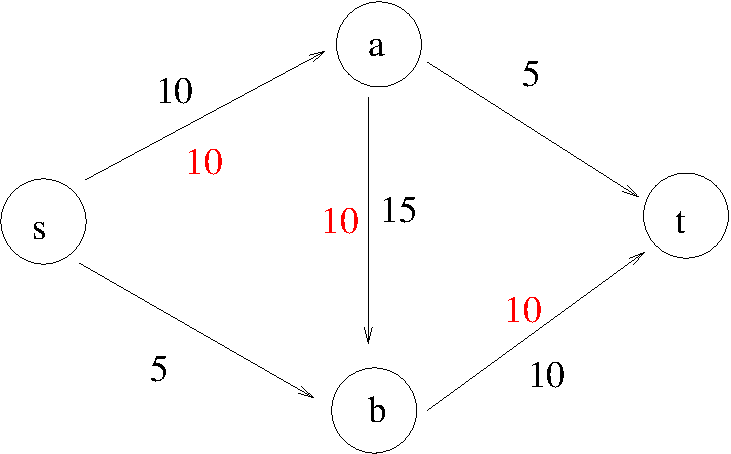
\includegraphics[width=6cm]{Figs/flow1.pdf} 
\hspace{1cm}
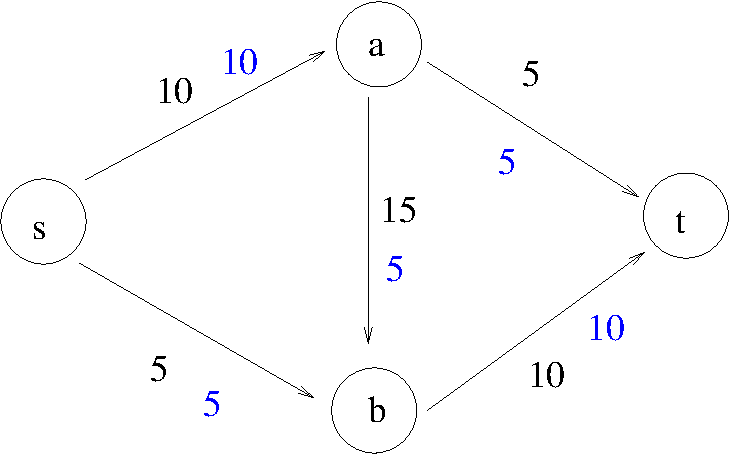
\includegraphics[width=6cm]{Figs/flow1b.pdf}
\end{center}
\caption{Left: Sample Flow (red) of value $10$ for a small network. Capacities are given in black. Right: Better Flow (blue) of value $15$.}\label{fig:flow1}
\end{figure}

Consider Figure \ref{fig:flow1},left, for an example of a valid flow (in red) for given edge capacities (in black). The value of this flow is $10$, no edge capacity is violated and at all nodes except for source and sink, the inflow equals the outflow.

How could we compute such a flow? A first attempt at an algorithm could be as follows:
\begin{verbatim}
   1. start with a zero-flow
   2. find a path consisting of edges with non-zero remaining capacities from s to t;
      send as much flow as possible across this path 
   3. repeat 2. as long as possible
\end{verbatim}
In step 2, the maximum amount of flow to be sent across a path is determined by its bottleneck -- the edge with smallest capacity along the path.
In fact, our algorithm might compute the flow depicted in Figure \ref{fig:flow1}, left, if the first path found was $s\rightarrow a\rightarrow b\rightarrow t$; then no further path of non-zero remaining capacities from $s$ to $t$ exists and the algorithm terminates. One important question remains open, though: Is the resulting flow optimal?

Unfortunately it turns out that it is not optimal. In Figure \ref{fig:flow1}, right, we see a flow (in blue) of value $15$, which could be the result of our algorithm (if the e.g. first the path $s\rightarrow a\rightarrow t$ followed by $s\rightarrow b \rightarrow t$ and $s\rightarrow a \rightarrow b \rightarrow t$ was picked) which could not be constructed from the flow on the left. So we better think of a refined algorithm.

The crucial observation that leads to an algorithm which actually computes a maximum flow can  be explained in Figure \ref{fig:flow1}, left. While there is no edge to send flow from $b$ to $a$, in presence of the red flow, there is still the possibility to send flow from $b$ to $a$ by \emph{sending less flow} from $a$ to $b$. In fact this corresponds to a virtual edge from $b$ to $a$ with capacity $10$ (since with the red flow being present, we can send at most $10$ units of flow less from $a$ to $b$).

Based on this observation we define for a given network $G(V,E,c)$ and flow $f:E\rightarrow \mathbb{R}^+$ the so-called \emph{residual network} $G_f(V, E_f, c_f)$ as follows:
\begin{itemize}
\item for any edge $e\in E$ with $c(e)>f(e)$ we have $e\in E_f$ with $c_f(e)=c)(e)-f(e)$
\item for any edge $e=(v,w)\in E$ with $f(e)>0$ we have an edge $e_R=(w,v)\in E_f$ with $c_f(e_R)=f(e)$
\end{itemize}
The first rule creates edges with non-zero remaining capacity in $G_f$, the second introduces all the virtual reverse edges for edges across which actual flow is sent. See Figure 6 for a flow in $G$ and the resulting residual network.
\begin{figure}
\begin{center}
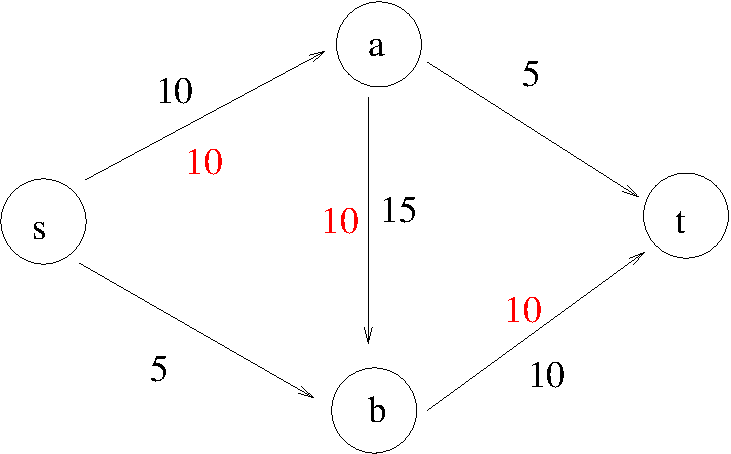
\includegraphics[width=6cm]{Figs/flow1.pdf} 
\hspace{1cm}
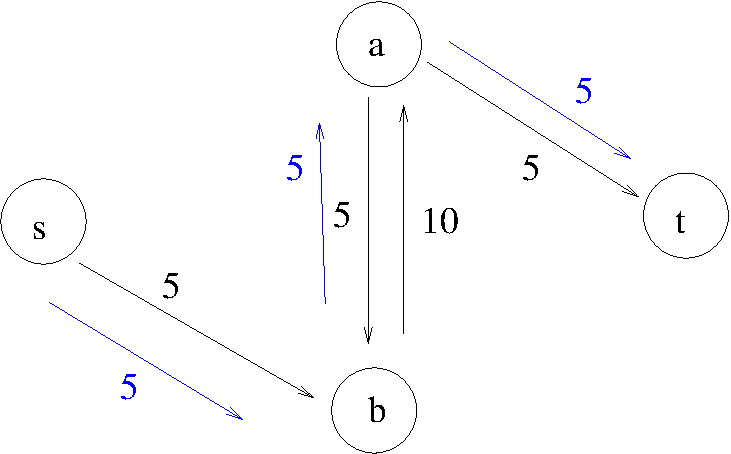
\includegraphics[width=6cm]{Figs/flowRN1.pdf}

\vspace{1cm}
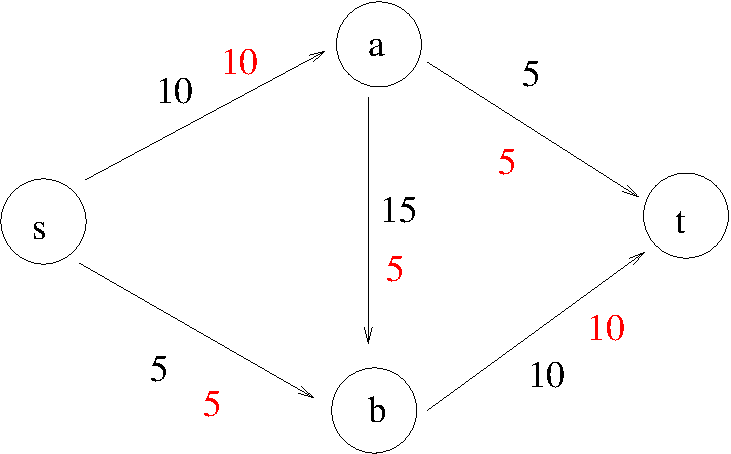
\includegraphics[width=6cm]{Figs/flowRN2.pdf}
\hspace{1cm}
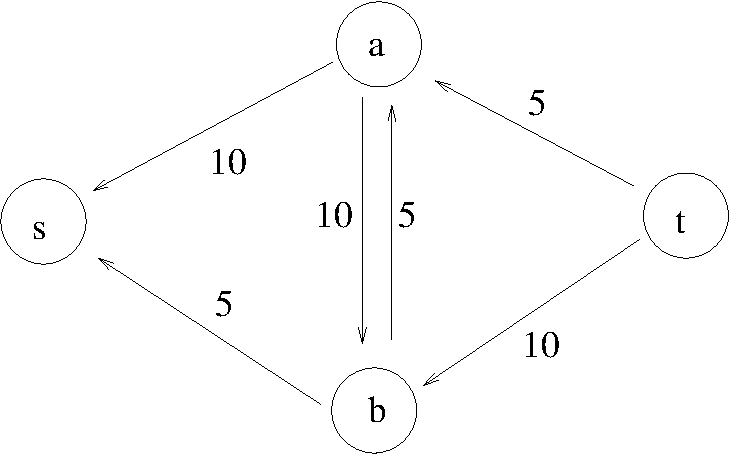
\includegraphics[width=6cm]{Figs/flowRN3.pdf}
\end{center}
\caption{Sample Flow (red) for a small network (upper left). Resulting residual network with possible augmenting path(upper right). Resulting total flow (lower left). Last residual network without $s$-$t$ path.}\label{fig:flowRN}
\end{figure}

Extending our first attempt at an algorithm in a natural way is then to search for $s$-$t$ paths in this residual network, sending flow across such a path (the amount of which is determined by the \emph{bottleneck} of the path, that is, its minimum capacity edge) if such exists, rebuilding the residual network etc. until no further path in the residual network exists. In fact this is the algorithm which we will be using and proving correctness for, it is called the \emph{Ford-Fulkerson} algorithm (google it!).	

\begin{verbatim}
   FORD-FULKERSON
   1. start with the zero-flow f=0
   2. Construct the residual network G_f
   3. find a path consisting of edges with non-zero remaining capacities 
       from s to t in G_f;
       send as muchflow as possible across this path; add this flow to f
       if no such path exists, stop the algorithm and return f
   4. goto 2.
\end{verbatim}

It is not hard to see that this algorithm (like the previous, incorrect one) terminates:

\begin{lemma}
The algorithm terminates in $\min\left(\sum_{e=(s,.)} c(e), \sum_{e=(.,t)} c(e)\right)$ steps.
\end{lemma}
\begin{proof}
In each round of the algorithm the net flow from $s$ to $t$ increases by at least $1$, hence
the total number of rounds is upper bounded by the sum of the outgoing capacities of $s$ and
the incoming capacities of $t$.
\end{proof}

For the new algorithm we can also prove that it computes indeed the maximum possible flow from $s$ to $t$.
To that end we first need a simple observation to derive upper bounds.

\begin{definition}
Let $G(V,E)$ be a directed graph, $A\subset V$  be a subset of the nodes.
The \emph{directed cut} induced by $A$ is defined as $\mbox{dcut}(A):=\{e=(v,w): v\in A, w\notin A\}$, that is,
the set of edges which have their source in $A$ and their target not in $A$.
\end{definition}

It is not hard to see that any such directed cut induces an upper bound on the maximum flow from $s$ to $6$
\begin{lemma}
For a directed graph $G(V,E)$ with edge capacities $c:E\rightarrow \mathbb{R}^+$ let $A\subset V$ be a subset of the nodes with $s\in A$, $t\notin A$, then $\sum_{e\in\mbox{dcut}(A)} c(e)$ is an upper bound on the max flow from $s$ to $t$.
\end{lemma}
\begin{proof}
Consider a maximum flow from $s$ to $t$; any unit of this flow has to cross the boundary from $A$ to $V-A$ somewhere. The amount of flow that can cross this boundary is bounded by the above quantity.
\end{proof}

The idea of our correctness proof is to consider the residual network of the final flow that our algorithm has produced and use this to exhibit a set $A$ inducing a directed cut which realizes an upper bound matching the flow our algorithm has produced.

To that end consider the set $A^*$ which consists of all nodes that are reachable from $s$ in the residual network $G_f$ of the flow $f$ that our algorithm has computed and consider the edges leaving and entering $A^*$.
\begin{lemma}
Let $f$ be the flow produced by our algorithm for a network $G(V,E)$ with edge capacities $c:E\rightarrow \mathbb{R}^+$, $e=(v,w)\in E$ with $\{v,w\}\cap A^*=1$. Then we have:
\begin{itemize}
\item if $v\in A^*$, that is, we have an edge $(v,w)$ out of  $A^*$, then $f(e)=c(e)$
\item if $w\in A^*$, that is, we have an edge $(v,w)$ into $A^*$, then $f(e)=0$ 
\end{itemize}
\end{lemma}
\begin{proof}
For the first part, observe that if $f(e)>0$, then there is an edge from $v$ to $w$ in the residual network of positive capacity making $w$ reachable from $s$ in $G_f$, contradicting the fact that $w\notin A^*$.
For the second part, note that if $f(e)>0$, then there is a back edge $(w,v)$ out of $A^*$ in $G_f$ with positive capacity, making $v$ reachable from $s$, also contradicting non-membership of $v$ in $A^*$.
\end{proof}

This almost concludes the correctness proof for the Ford-Fulkerson algorithm. Due to the previous Lemma we know that the value of the flow $f$ produced is $\displaystyle \sum_{e=(v,w): v\in A^*, w\notin A^*} f(e)=\sum_{e=(v,w): v\in A^*, w\notin A^*} c(e)$, but as the directed cut induced by $A^*$ implies an upper bound of\\ $\displaystyle\sum_{e=(v,w): v\in A^*, w\notin A^*} f(e)$, the two bounds match and we have shown optimality of $f$.

\begin{corollary}
The Ford-Fulkerson algorithm terminates and computes a maximum flow.
\end{corollary}

Note that the running time of Ford-Fulkerson in this version can only be bounded by $O(C(n+m))$ where $C$ denotes the sum of capacities. $O(m+n)$ time is required for each construction of the residual network and construction of an augmenting path. Unfortunately $C$ might not be polynomial in the input size. See Figure \ref{FIG:FFbad} for an example where FF might take a very long time (for a bad sequence of augmenting paths).

\begin{figure}
\centering
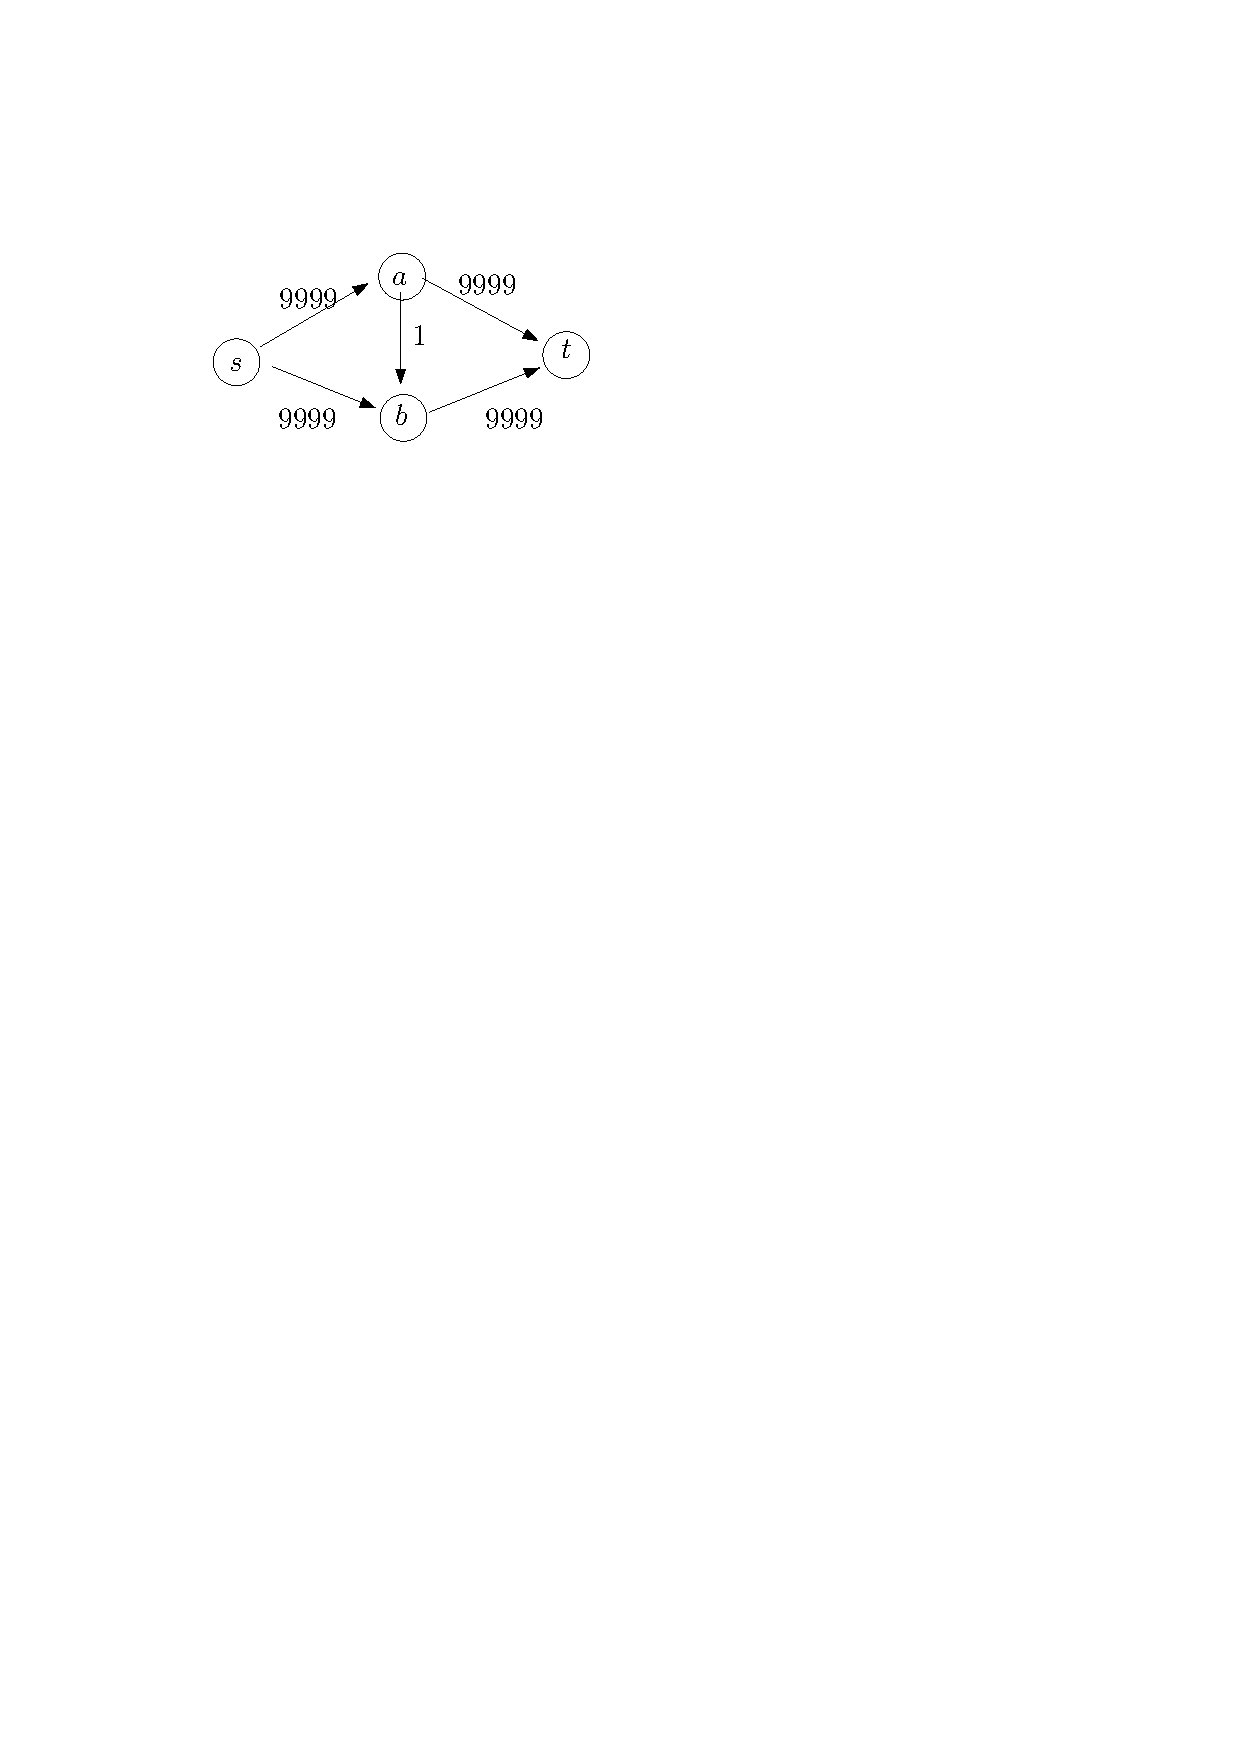
\includegraphics[width=6cm]{Figs/FF-bad.pdf}
\caption{Example where FF might take a long time.}\label{FIG:FFbad}
\end{figure}

\subsubsection{Capacity Scaling}
In the following we will describe a modification of the original FF algorithm that allows to prove a polynomial running time. The idea is first to search for augmenting paths with large bottlenecks only, and only if such paths cannot be found anymore, search for augmenting paths with smaller bottlenecks. The algorithm can be described as follows:
\begin{verbatim}
	start with a zero-flow f
	D= next smaller power of two of max capacity
	while (D>=1) do
	   Gf=residual network of G wrt f restricted to edges of capacity >=D
	   while there is an augmenting path in Gf do
	      augment f, recompute Gf
	   done
	   D=D/2
	done
\end{verbatim}

Observe that the algorithm certainly terminates and produces a maximum flow as each augmentation increases the flow by at least $1$ and when $D=1$, $G_f$ is the residual network as in the original Ford-Fulkerson algorithm.
Let us try to argue now that the number of augmentations is polynomially bounded.
Note that the outer loop is executed $O(\log C)$ times where $C$ denotes the maximum capacity of an edge in the network.

\begin{lemma}
Let $f_D$ be the flow after completing augmentations with capacity value $D$. Then the maximum flow of the network is bounded by $val(f_D)+mD$.
\end{lemma}
\begin{proof}
Consider the residual network $G_{f_D}$ after the last augmentation with capacity value $D$ (including all edges with capacity less than $D$). Let $A$ be the set of nodes reachable from $s$ if all edges of capacity $<D$ are removed from $G_{f_D}$. $A$ induces a directed cut of some capacity $C$. If we subtract the current flow $f_D$ from the edge capacities of the edges leaving $A$, we know that all these edges have remaining capacity $<D$. There can be at most $m$ such edges, hence the $C-val(f_D)<mD$.
\end{proof}

\begin{lemma}
For fixed $D$, the inner while loop is executed at most $2m$ times.
\end{lemma}
\begin{proof}
Starting with a flow $f$ for fixed $D$, we know (from the previous round with $2D$ that the total flow is bounded by $val(f)+2Dm$. In each round of the inner while loop, the flow is increased by at least $D$, hence there can be at most $2m$ round of the inner while loop.
\end{proof}

\begin{theorem}
Ford-Fulkerson with capacity scaling terminates after $O(2m(m+n)\log C)=O(m^2\log C)$ steps.
\end{theorem}

\subsubsection{Shortest Augmenting Path (Edmonds-Karp Algorithm)}
Capacity scaling leads to a running time guarantee which still depends on the magnitude of the capacities.
In the following we will show that when augmenting always using a \emph{shortest} path (in terms of hop distance), the running time can be bounded by $O(m^2n)$.

So consider in the following the variant of Ford-Fulkerson, where we always augment on a \emph{shortest path} in the current residual network $G_f$. Such a shortest path can be computed using Breadth-First-Search in $O(m+n)$.

We will prove the following two lemmas 
\begin{lemma}\label{lem:SPnondec}
During the course of the algorithm, the length of the augmenting paths never decreases.
\end{lemma}
\begin{lemma}\label{lem:SPinc}
After at most $O(m)$ augmentations, the length of the augmenting path increases by at least one.
\end{lemma}

The two lemmas immediately lead to the following theorem:
\begin{theorem}
Ford-Fulkerson with shortest-path augmentation terminates after $O(m^2n)$ steps.
\end{theorem}

Let us prove the two lemmas in the following:
\begin{proof}(Lemma \ref{lem:SPnondec})
Let $l(v)$ be the distance of $v$ from $s$ in the residual network. $G_l$ the subgraph of residual network which only contains edges $(u,v)$ with $l(v)=l(u)+1$. A path $\pi$ in the residual network is a shortest path if it is a path in $G_l$. When augmenting along a path $\pi$, two things can happen along this path: (a) edges in the residual network disappear (as their capacity is fully used up) or (b) back edges are created which have not been present before. None of these modifications to the residual network can increase the level of any node, though. Therefore, the distance to any node -- in particular also to $t$ -- never decreases.
\end{proof}

\begin{proof}(Lemma \ref{lem:SPinc})
Let $E_k$ be the set of edges at the beginning of a phase when the distance between $s$ and $t$ is $k$. As soon as the shortest path from $s$ to $t$ uses an edge not in $E_k$ it has length larger $k$. Since with every augmentation, at least one edge (the bottleneck edge) is eliminated from $E_k$, after at most $m$ steps, the length of the shortest path from $s$ to $t$ must increase.
\end{proof}

\subsubsection{Non-integral Capacities}
So far we have always assumed \emph{integral} edge capacities, our termination and running time argumentation crucially relied on that. If edge capacities are real numbers, though, termination cannot be guaranteed and there are simple examples where Ford-Fulkerson not even converges towards the maximum flow (google it!).



\subsection{MinCostFlow}
Let us now consider an extension of the maxFlow problem where we also have to take into account \emph{costs}.
So we are given a directed network $G(V,E)$ with capacities $cap:E\rightarrow \mathbb{N}$ and costs $c:E\rightarrow \mathbb{Z}$. Furthermore, we have a function $b:V\rightarrow \mathbb{Z}$ which determines whether a node $v$ has a supply/surplus of flow ($b(v)>0$) or a demand of flow ($b(v)<0)$; there might also be nodes which only act as relays ($b(v)=0$).

We assume that the surplus equals the demand, that is, $\displaystyle \sum_{v:b(v)<0} b(v)=-\sum_{v:b(v)>0} b(v)$.
The goal of the minCostFlow problem is to determine a flow $f:E\rightarrow \mathbb{N}$ such that
\begin{itemize}
\item $\forall e\in E: 0\leq f(e)\leq cap(e)$ (flow on an edge does not exceed the capacity)
\item $\forall v\in V$: $\displaystyle b(v)+\sum_{e=(w,v)}f(e)=\sum_{e=(v,w)}f(e)$ (incoming and outgoing flow together with the surplus/deficit of the vertex balance out)
\item $\displaystyle\min \sum_{e\in E} f(e)c(e)$ (minimizing the total cost of the flow)
\end{itemize}

See Figure \ref{fig:minCostFlow-Ex1} for an example of a mcf instance as well as a feasible, but possibly not cost-optimal flow.

\begin{figure}
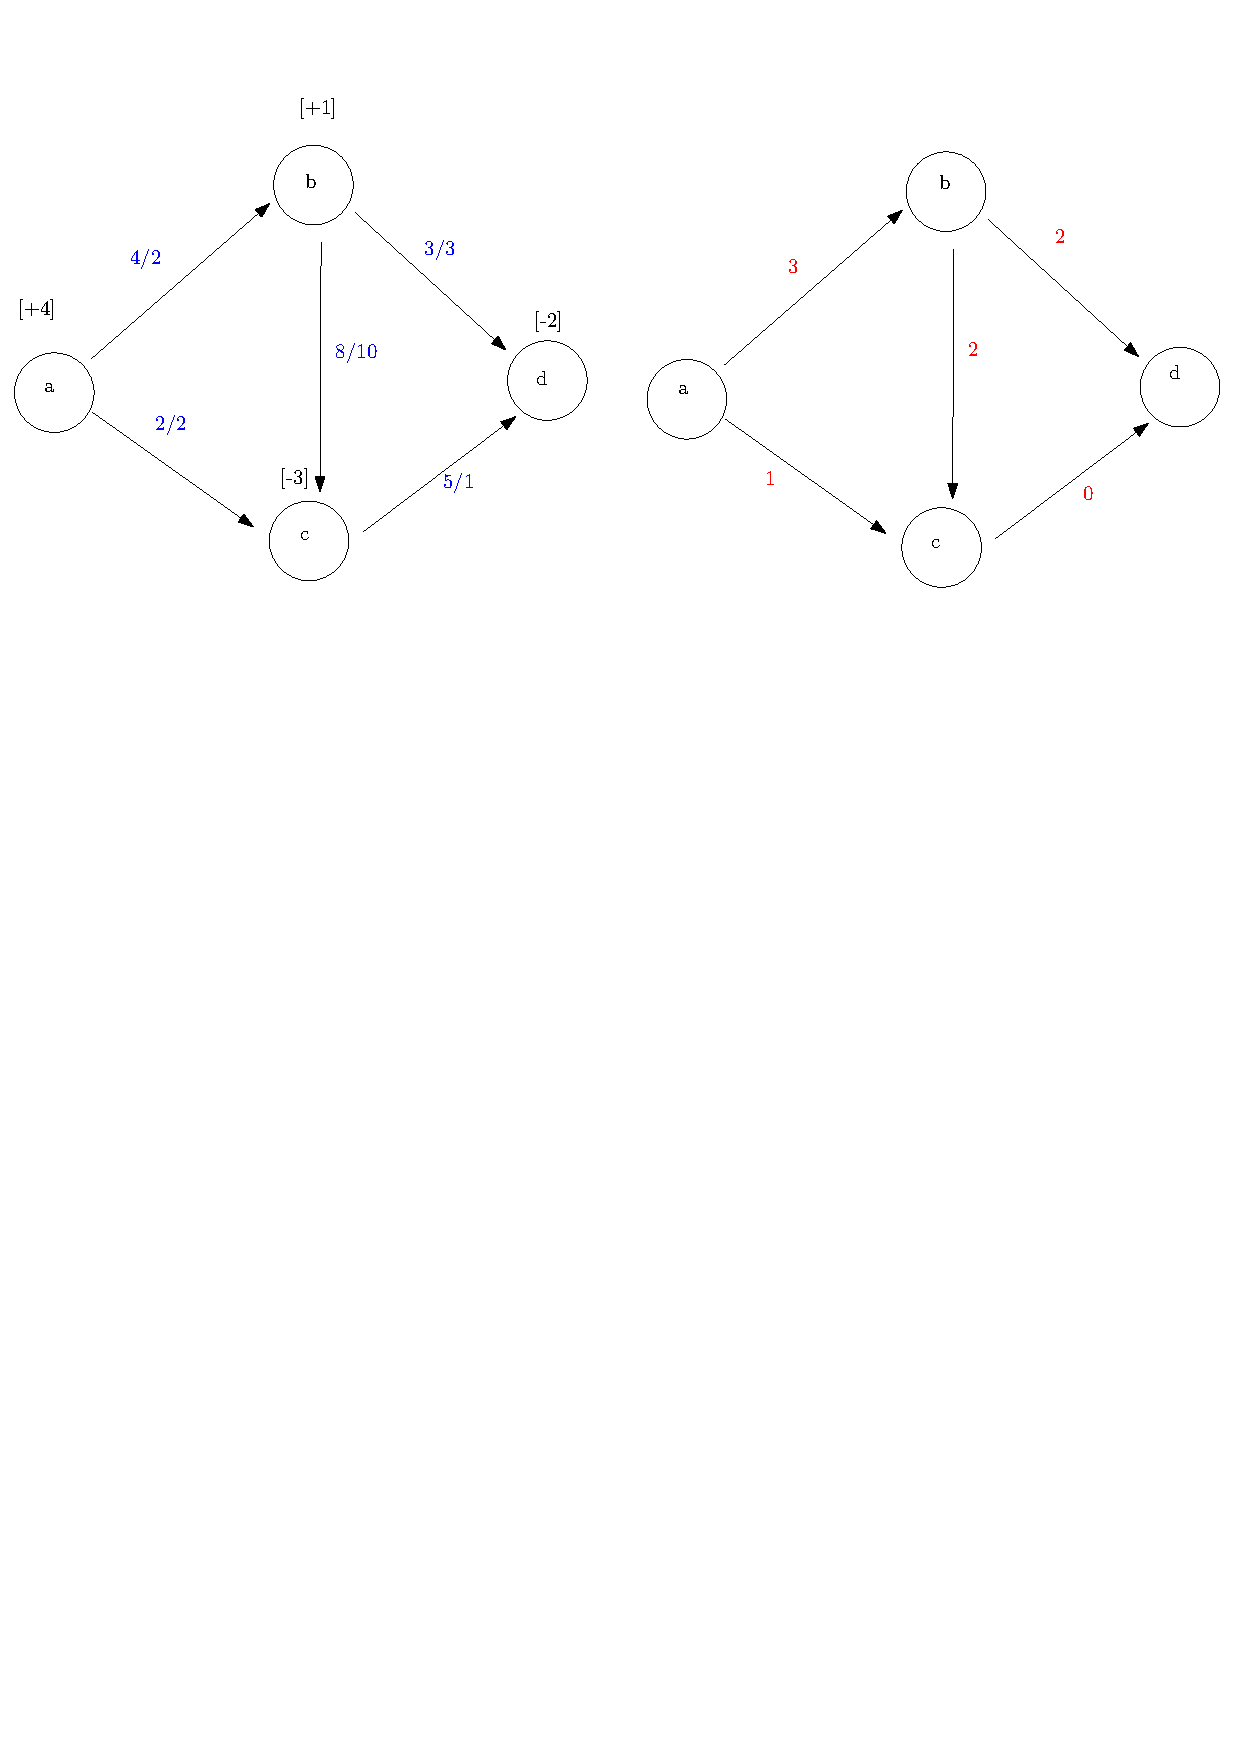
\includegraphics[width=\textwidth]{Figs/minCostFlow-Ex1.pdf}
\caption{MinCostFlow instance on the left; demand/surplus in brackets at the nodes, capacities/costs written at the edges. Feasible flow on the right (in red) of cost 34.}\label{fig:minCostFlow-Ex1}
\end{figure}

\subsubsection{MinCostFlow via Cycle Cancelling}
Note that it is easy to obtain a \emph{feasible} flow  via a single maxFlow computation: create a supersource $s$ which has an edge to each node $v\in V$ with $b(v)>0$ with capacity $b(v)$, and a supersink $t$ which has an incoming edge from each $v\in V$ with $b(v)<0$ with capacity $-b(v)$. A feasible flow exists iff the respective maxFlow has value $\sum_{v:b(v)>0} b(v)=\sum_{v:b(v)<0}-b(v)$.
So let us assume that we have a feasible flow and we want to decrease its cost.

We proceed quite similar as for maxFlow in that we consider the \emph{residual network} $G'(V,E')$ for a given network $G(V,E)$ and a flow $f$. For each edge $e=(v,w)\in E$ with cost $c(e)$ and capacity $cap(e)$ we construct up to two edges $e_1, e_2$ in $E'$ as follows:
\begin{itemize}
\item if $f(e)<cap(e)$ there is an edge $e_1=(v,w)$ with cost $c'(e_1)=c(e)$ and capacity $cap'(e_1)=cap(e)-f(e)$
	(a forward edge with the remaining capacity)
\item if $f(e)>0$ there is an edge $e_2=(w,v)$ with cost $c'(e_1)=-c(e)$ and capacity $cap'(e_2)=f(e)$ (a backward edge with negative cost and capacity equal to the forward flow)
\end{itemize}

In Figure \ref{fig:minCostFlow-Ex1-residual}, left we see the respective residual network for the above problem instance and flow. 

\begin{figure}
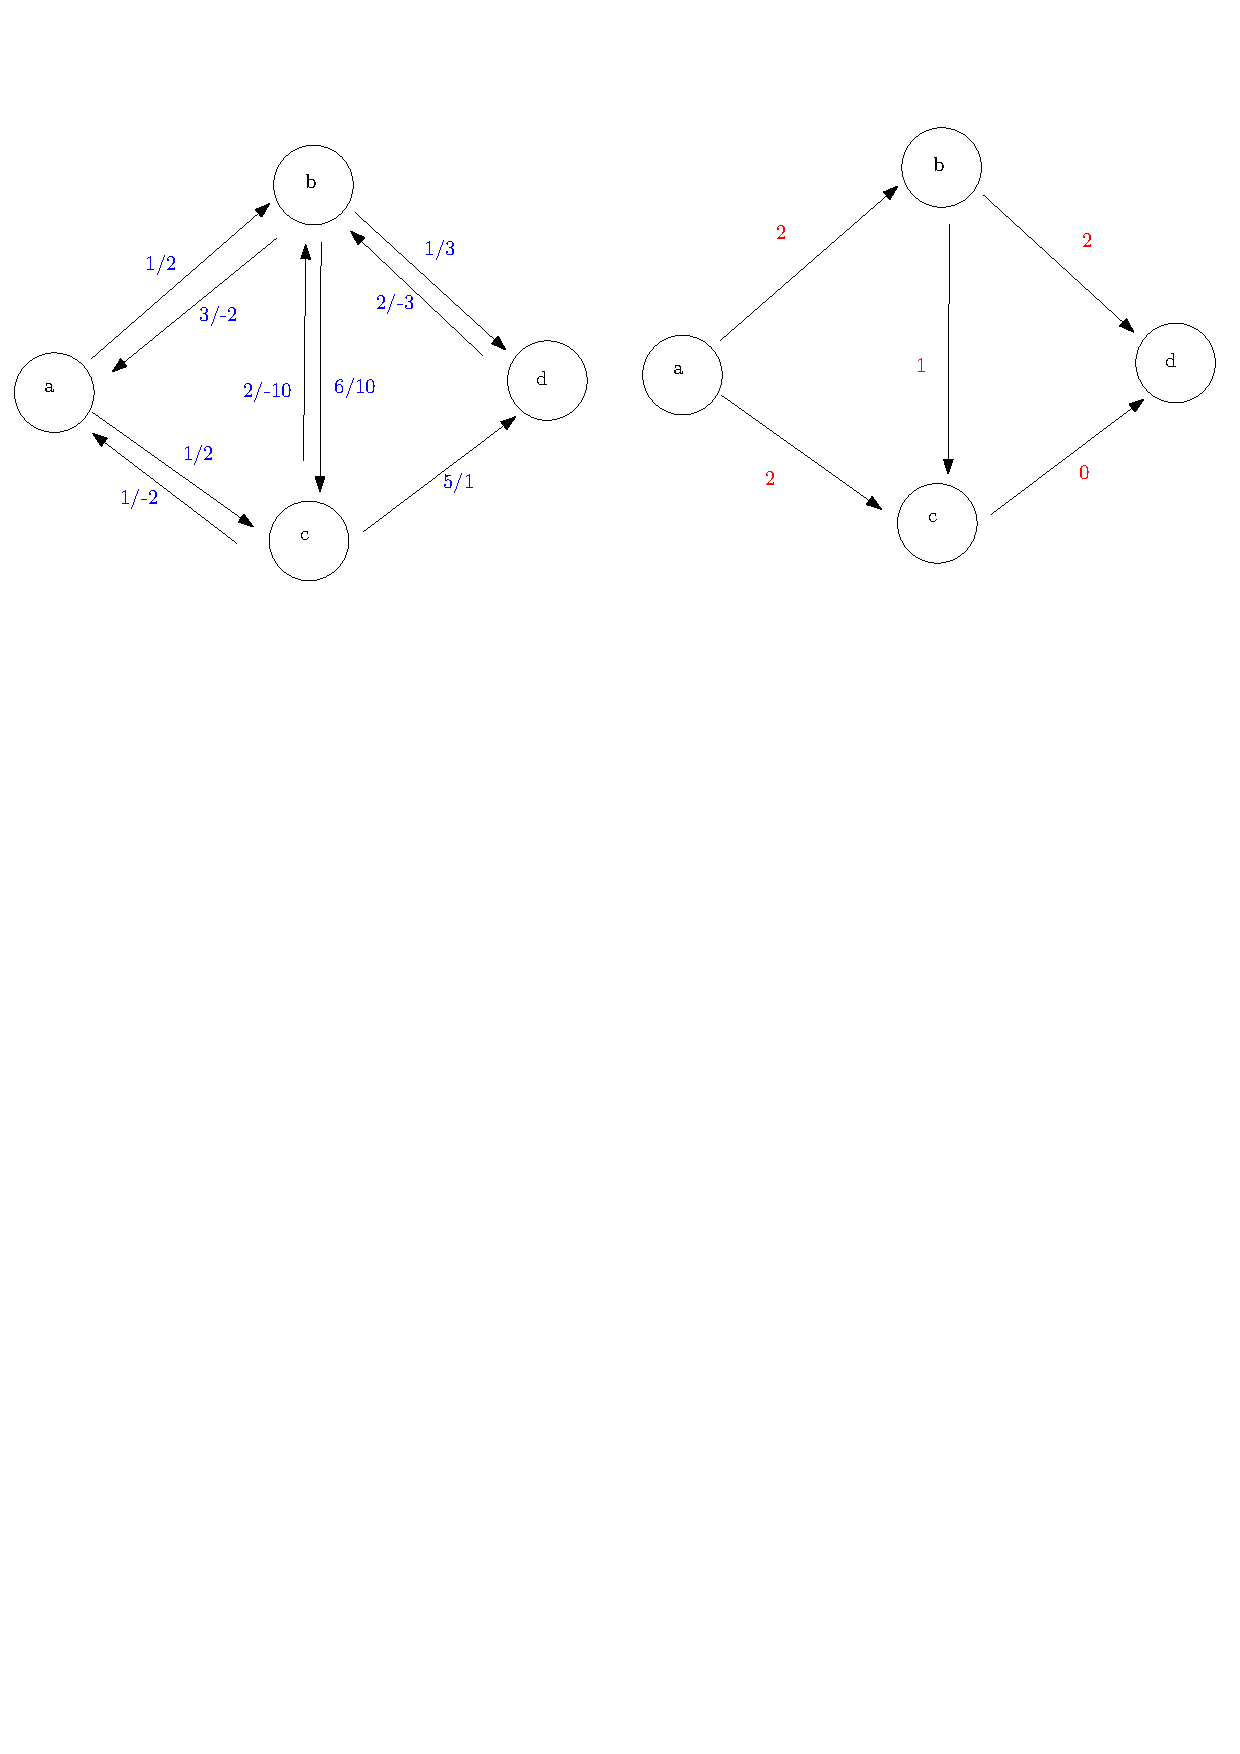
\includegraphics[width=\textwidth]{Figs/minCostFlow-Ex1-residual}
\caption{Residual network for mcf instance and flow from Figure \ref{fig:minCostFlow-Ex1} (left). Resulting flow of cost 24 after sending one unit of flow along the negative cycle cbac (right).}\label{fig:minCostFlow-Ex1-residual}
\end{figure}

\begin{figure}
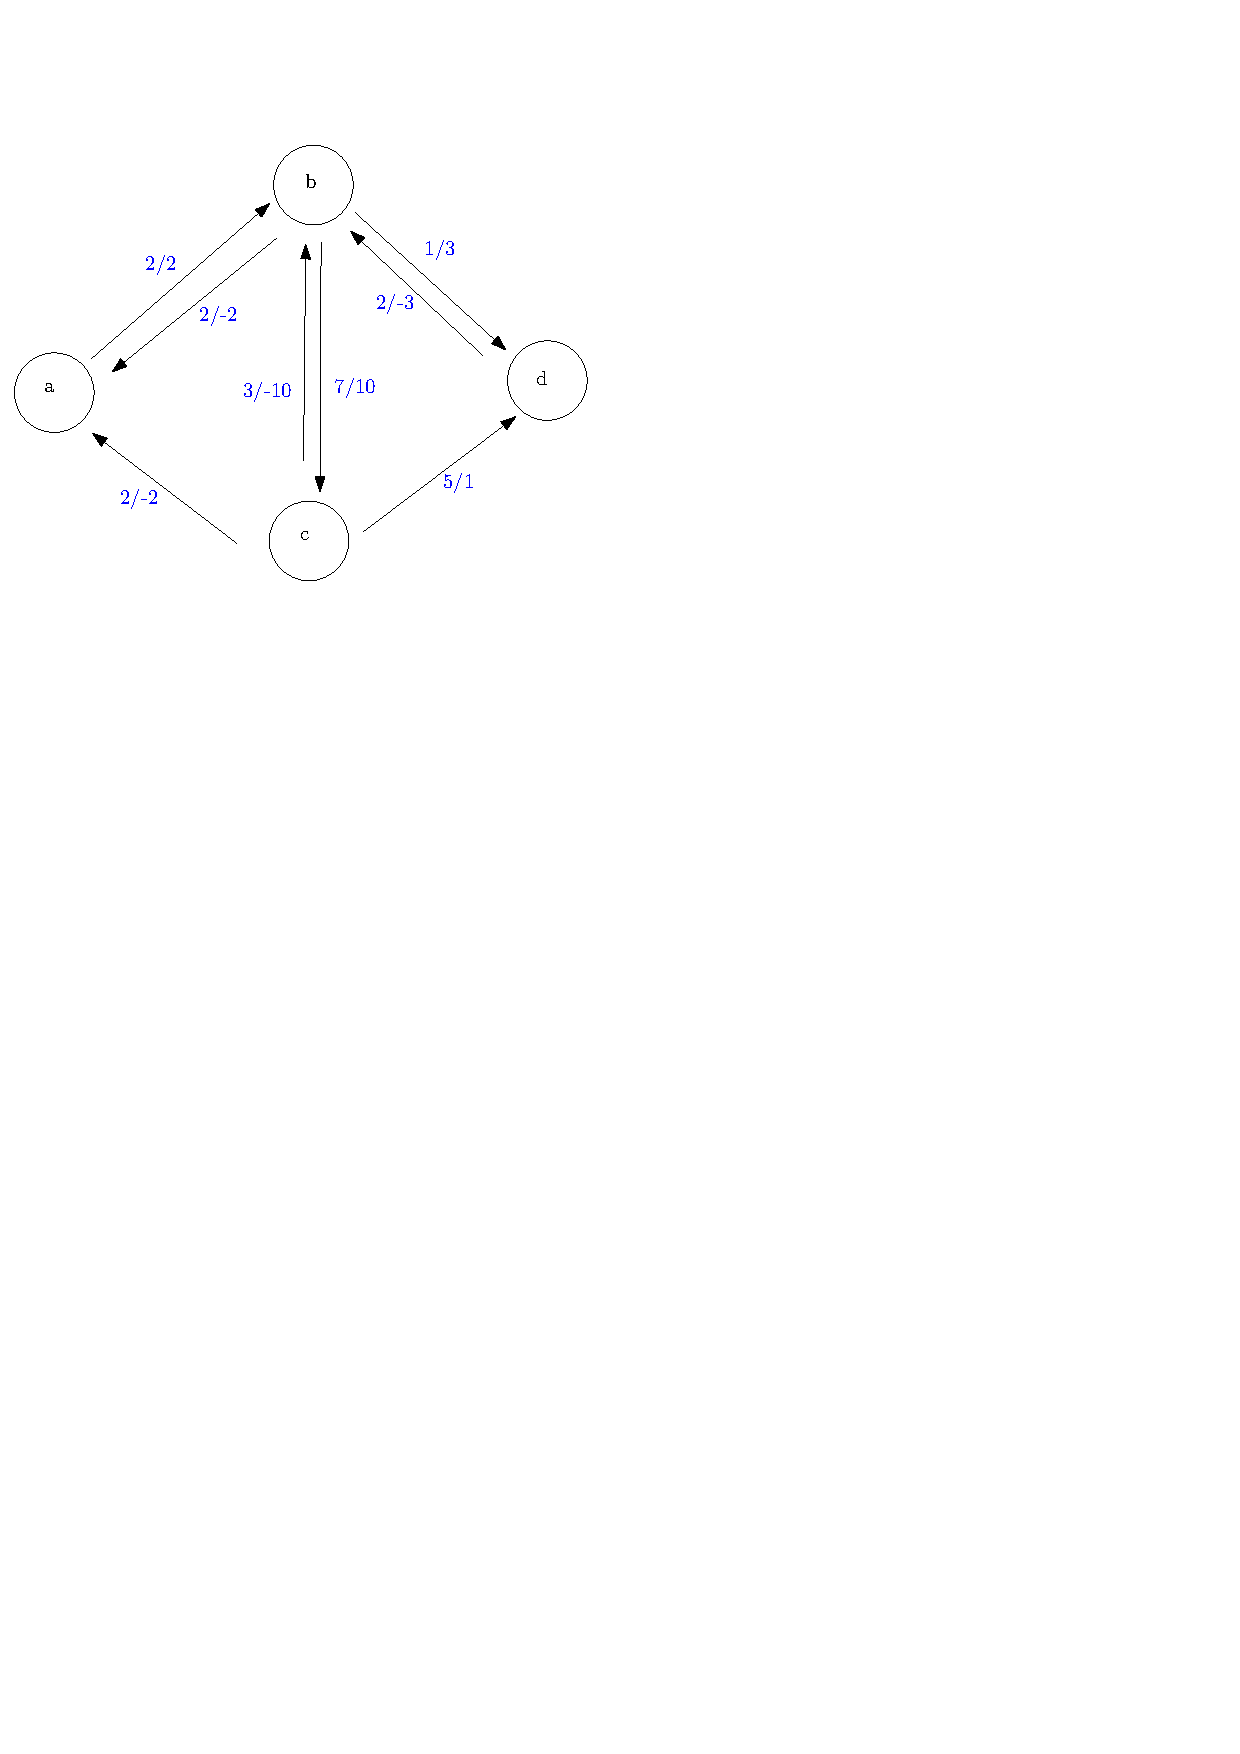
\includegraphics[width=0.5\textwidth]{Figs/minCostFlow-Ex1-residual2}
\caption{Final residual network without negative cycles.}\label{fig:minCostFlow-Ex1-residual2}
\end{figure}

While in our maxFlow algorithm we were looking for $s$-$t$-paths in this residual network, here we are looking for \emph{negative cycles}, that is a sequence of adjacent edges which ends up in the starting vertex and has negative cost in total. We send as much flow around this cycle as possible (as determined by the bottleneck edge capacity), hereby decreasing the total cost of the flow.

In the residual network in Figure \ref{fig:minCostFlow-Ex1-residual}, left there exists a cycle $cbac$ of negativ cost; sending one unit of flow along this cycle (more is not possible due to the bottleneck edge $(a,c)$) decreases the total cost resulting in the flow in Figure \ref{fig:minCostFlow-Ex1-residual}, right.


As in Ford-Fulkerson we repeat this procedure until no negative cycles can be found in the residual network. As we will prove in the following, the resulting flow has to be optimal.

In Figure \ref{fig:minCostFlow-Ex1-residual2} we see the residual network for the updated flow. This network does not contain any negative cycle, so the flow is hopefully cost-optimal.

\begin{lemma}
Let $f$ be a flow in $G$, $G_f$ the respective residual network. Then, $f$ is a minCost flow if and only if $G_f$ does not contain any negative cycle.
\end{lemma}
\begin{proof}
The '$\Rightarrow$'-direction is trivial, so let us focus on the other direction and assume $G_f$ does not contain any negative cycle but $f$ is not a minCost flow. We will derive a contradiction hence proving the lemma.

Let $f^*$ be a minCost flow and consider the flow difference $f'=f^*-f$. We claim $f'$ has to contain a negative cycle. Clearly we have $c(f')<0$ since $c(f^*)<c(f)$. Furthermore, note that for $f'$ flow conservation must hold, that is, at any $v\in V$ the inflow and the outflow of $f'$ balances out to $0$. Therefore, $f'$ must be decomposable into a set of one or more \emph{cycles}. Since the total cost of the cycles is negative, one of the cycles must have negative cost. Let that cycle be $C$; note that the flow described by $C$ can also be sent around in $G_f$, contradicting the fact that $G_f$ has no cycle of negative cost.
\end{proof}

So, as long as the current flow $f$ is not optimal, we will find a negative cycle in $G_f$, hence decreasing the cost of the flow by at least $1$ (for integral capacities and costs). Termination and correctness follow.

\subsubsection*{Detection of Negative Cycles}
How can we detect negative cycles in a graph $G(V,E,c)$? A naive way of doing so is to construct the following \emph{layered graph}:
we have $n$ layers where each layer contains the node set $v_1, \dots, v_n$. We have an edge between $v_i$ and $v_j$ in the next
layer if there is an edge $(v_i, v_j)\in E$ (of the same cost), see Figure \ref{fig:negCycle}. Now, we can compute shortest path distances for each $v_i$ in layer $1$ to the $v_i$ in the other layers in $O(mn)$ time each. If there is a negative cycle in $G$, it will be exhibited.
\begin{figure}
\begin{center}
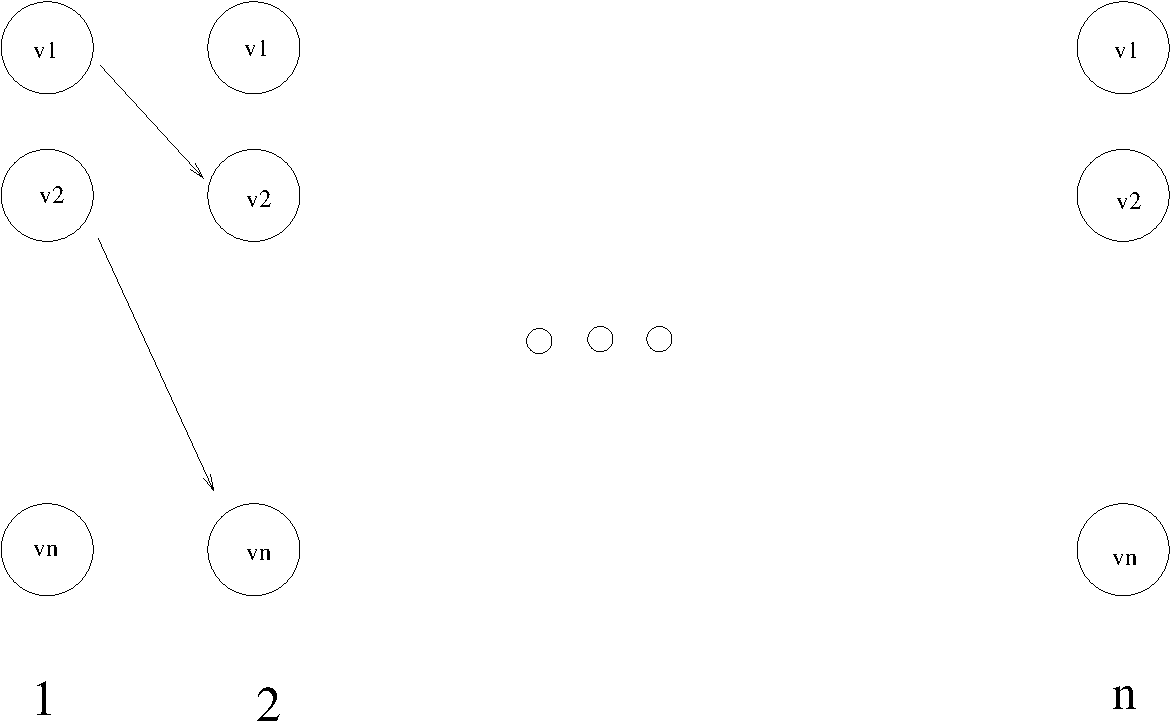
\includegraphics[width=0.5\textwidth]{Figs/negCycle.pdf}
\caption{Layered graph construction to detect negative cycles.}\label{fig:negCycle}
\end{center}
\end{figure}

While this naive approach requires $O(mn^2)$ steps it is also possible to employ Bellman-Ford and exhibit a negative cycle in time $O(mn)$ or conclude that no negative cycle exists.

In fact, when we always look for the negative cycle $C$ which minimizes $c(C)/|C|$, one can even prove that after polynomially many cycle detections the mincost flow has been found (similar to the maxFlow case where we used a specific rule to determine augmenting paths which guaranteed polynomial running time).



\subsubsection{MinCostFlow via Successive Shortest Paths (sketch)}
While the idea of cycle cancelling was to start with a \emph{feasible maxFlow} and decrease its cost by repeatedly identifying cycles of negative cost in the residual network, another strategy is to start with a zero flow and iteratively augment this flow while maintaining cost optimality. This is done by computing a  shortest augmenting path (\emph{wrt to the edge costs}) from some supply node to some demand node in the current residual network and sending as much flow as possible across that path. Then the supply and the demand of the respective nodes are reduced and the residual network is updated.
 Cost optimality (even for a non-maximal flow) is certified by absence of negative cycles in the residual network (we will argue that this is the case). Termination and construction of a feasible maxflow is guaranteed for the same reason as for the Ford-Fulkerson algorithm -- indeed, we can view this simply as a specific strategy for picking augmenting paths in the Ford-Fulkerson algorithm which happens to guarantee cost optimality.
 
How can we find the shortest path from some supply to some demand node? We construct a super source $s$ and connect this with outgoing edges of inifinite capacity and zero cost to all supply nodes, and a super sink $t$ which has incoming edges from all demand nodes (also with infinite capacity and zero cost). Then we compute a shortest path from $s$ to $t$ wrt to the edge costs e.g. using Bellman-Ford. 

\begin{figure}
\centering
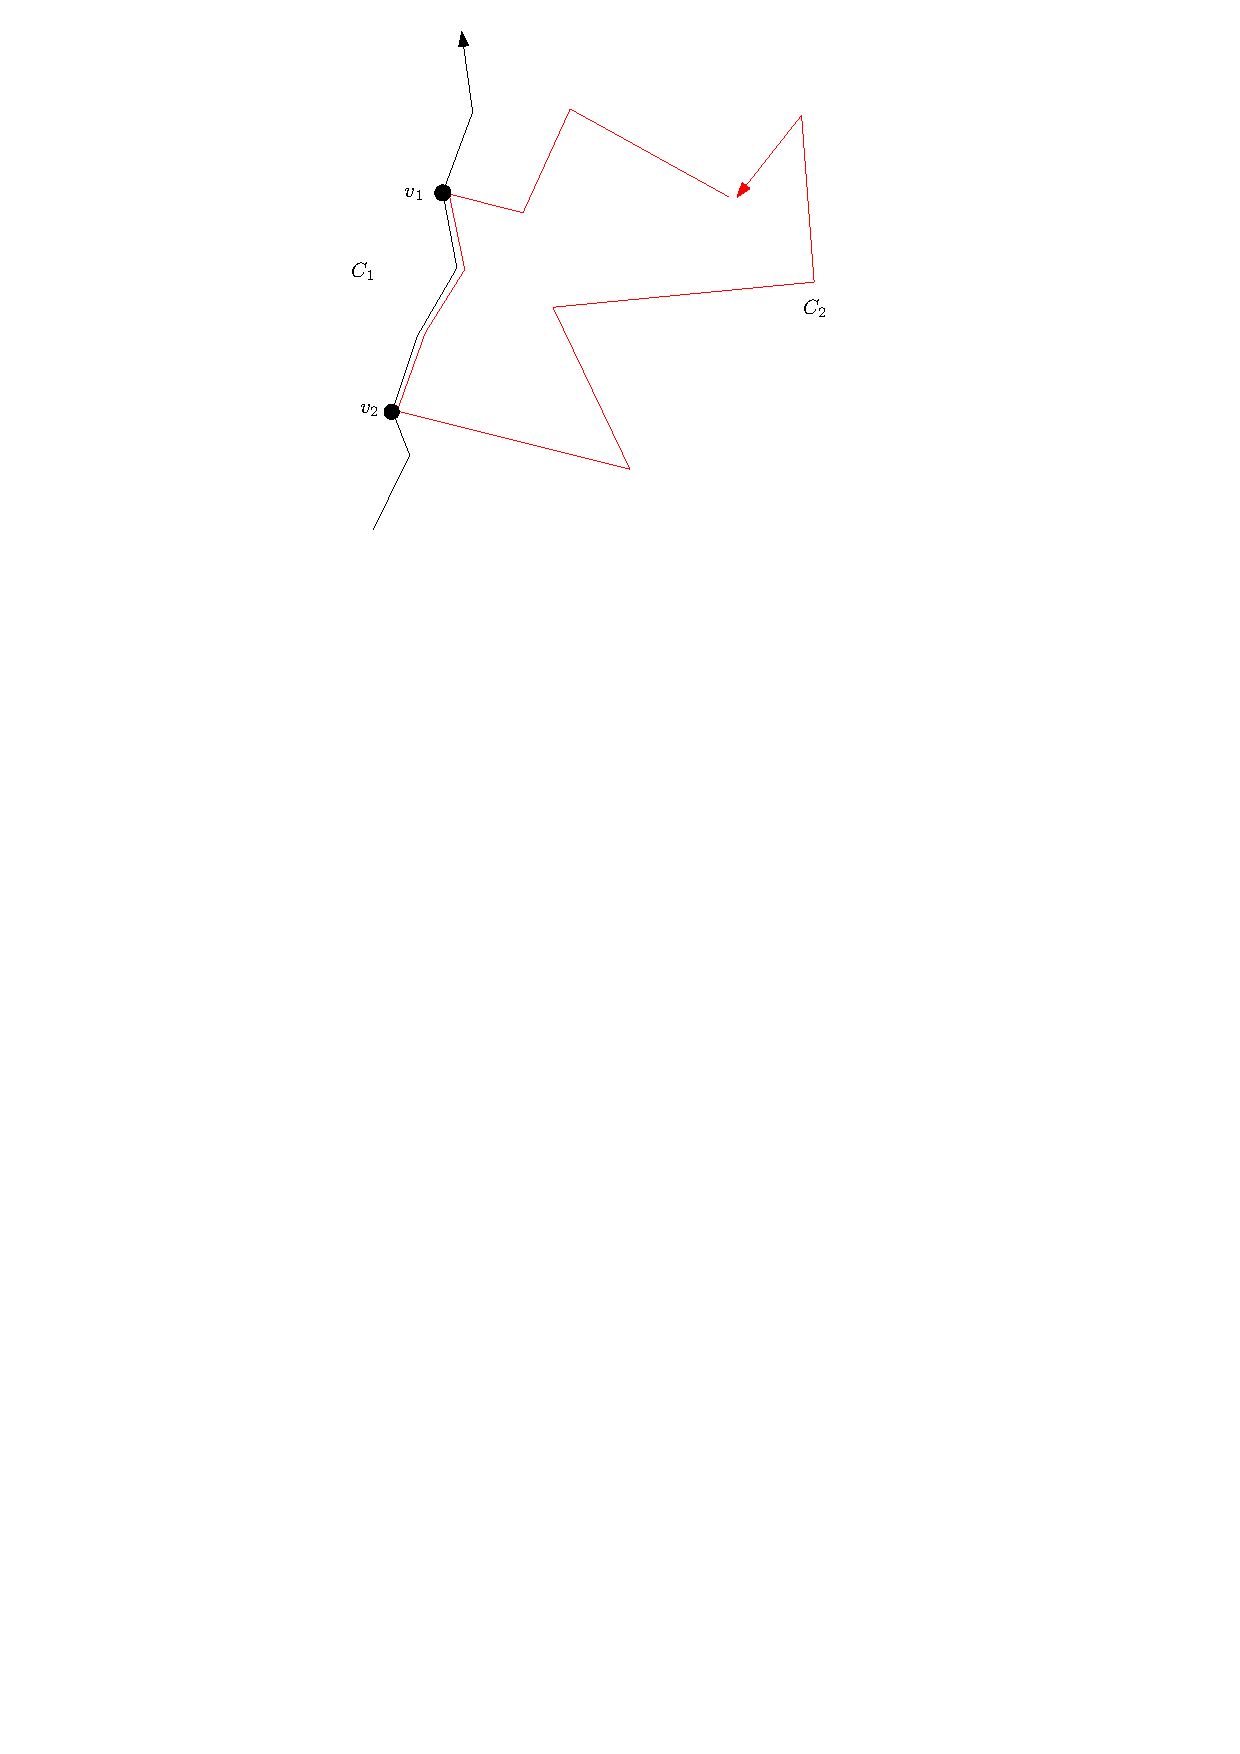
\includegraphics[width=0.4\textwidth]{Figs/SSP-noNegCyc.pdf}
\caption{Augmenting path in black, negative Cycle $C=C_1.C_2$. $C_1$ traverses the augmenting path between $v_2$ and $v_1$ in reverse direction (negative costs!).}\label{fig:SSPnoNegCyc}
\end{figure}
How can we argue that after sending the maximum amount of flow across the identified augmenting path, the new residual network remains free of negative cycles? To that end, let us consider the first residual network (wrt to a zero flow) which has only positive edge costs. After augmentation, the only negative edge costs appear as reverse edges along the augmenting path. If after the augmentation a negative cycle $C$ exists, $C$ can be decomposed into paths $C_1$ and $C_2$ where $C_1$ starts and ends with negative cost edges and $C_2$ only contains positive cost edges. The cost of $C_1$ must be negative, the cost of $C_2$ positive and $|cost(C_1)|>|cost(C_2)|$. Assume $C_1$ starts in $v_1$ and ends in $v_2$.  W.l.o.g. $C_1$ only consists of a continuous reverse subpath from $v_1$ to $v_2$ of the augmenting path (needs some argument $\Rightarrow$ exercise), that is, its cost is the (negative) cost of a subpath from $v_2$ to $v_1$ in the augmenting path, see the illustration in Figure \ref{fig:SSPnoNegCyc}. Observe that $C_2$ also yields a path from $v_2$ to $v_1$ with $|cost(C_2)|<|cost(C_1)|$ which contradicts the fact that the reverse of $C_1$ was a shortest path in the first residual network. So we can be sure that after the first augmentation the respective residual network is free of negative cycles. 

How can we extend this observation to the following residual networks? Here, an old result by Johnson comes as a rescue:

\begin{theorem}[Johnson]
Let $G(V,E,c)$ be a directed, weighted graph with possibly negative edge costs $c:E\rightarrow \mathbb{Z}$, but without negative cycles. Then there exists a potential function $\phi:V\rightarrow \mathbb{Z}$ such that the shifted edge costs $c'(v,w)=c(c,w)+\phi(v)-\phi(w)$ is always non-negative and shortest paths in $G(V,E,c)$ remain shortest paths in $G(V,E,c')$ and vice versa.
\end{theorem}
\begin{proof}
W.l.o.g. assume that $\exists s\in V$ from which all other nodes in $G$ can be reached. If $G(V,E,c)$ does not contain negative cycles, shortest path distances from $s$ are well-defined and can be computed using e.g. Bellman-Ford in $O(mn)$ time. Let us then define $\phi(v):=d_s(v)$ for all $v\in V$, that is, simply the shortest path distance from $s$. First, observe that due to $d_s$ being shortest path distances, $\forall (v,w)\in E$ we have $d_s(w)\leq d_s(v)+c(v,w)$ (otherwise going from $s$ to $w$ via $v$ yields a path shorter than $d_s(w)$). This is equivalent to $d_s(v)-d_s(w)+c(v,w)\geq 0$ or in other words $\phi(v)-\phi(w)+c(v,w)\geq 0$, that is, the new edge cost function $c'$ is always non-negative. Second, consider some path $\pi=sv_0v_1\dots t$ in $G(V,E,c')$; the cost of the path is $\sum_{(v,w)\in \pi} c'(v,w)=\sum_{(v,w)\in \pi} \phi(v)-\phi(w)+c(v,w)=\phi(s)-\phi(t)+\sum_{(v,w)\in\pi}c(v,w)$, that is, its original cost plus the potential of the source minus the potential of the target. Since the latter two terms are invariant for different $s-t$-paths, shortest paths in $G(V,E,c)$ are shortest in $G(V,E,c')$ and vice versa.
\end{proof}


So we can turn the second residual network (after the first augmentation) again into a network which has only non-negative edge costs and repeat the argument. In fact, most descriptions of the successive shortest path approach for MinCostFlow immediately apply the respective potential changes in the algorithm -- they might obscure the basic idea of the algorithm, though. The transformation into a graph with non-negative edge costs also allows for the application of Dijkstra's algorithm for finding the shortest paths along which to augment the flow.

\subsection{Applications of Flow}
There are many other interesting real-world problems -- apart from direct flow problems -- that can be modeled as a flow optimization problem. In the following we give some examples. 

\subsubsection{(MinCost) Bipartite Matching}
Consider a set of Jobs $J$ and a set of workers $W$ with $|J|=|W|=n$. Each worker $w\in W$, due to his qualification, is able to process a certain subset $J_w\subset J$ of tasks. Is it possible to find an assignment of jobs to workers such that every job is processed and no worker has to process more than one job?

This problem can be modelled as a maxFlow problem instance by creating a network with $V=W\cup J\cup\{s,t\}$ and edges $(w,j)$ of capacity $1$ between $w\in W$ and $j\in J$ if worker $w$ can process job $j$. Additionally we have capacity $1$ edges $(s,w)$ for all $w\in W$ and $(j,t)$ for all $j\in J$. A 1:1 assignment of jobs now exists iff the max flow from $s$ to $t$ is $n$.

A generalization of this problem where each job-worker pair has an associated processing time and the goal is to minimize the sum of processing times can be modelled as a minCostFlow problem.

\subsubsection{Edge Connectivity Edge-Disjoint Paths}
Given an undirected graph, its \emph{edge connectivity} $ec(G)$ is the minimal number of edges that need to be removed to make the graph disconnected. Clearly $ec(G)\leq \min deg(v)$, since removing all adjacent edges of a node makes $G$ disconnected. The edge connectivity of $G$ might be much smaller than the minimum degree of the nodes of $G$, though.

We can determine the edge connectivity by creating a network where each undirected edge is replaced by two directed edges of capacity $1$ (back and forth). We then compute the maxFlow from some fixed node $s$ to each $v\in V-\{s\}$. The minimum over all the flow values is the edge connectivity.

Similarly, for given $s$ and $t$ we might be interested in the number of \emph{edge disjoint} paths between $s$ and $t$. This number can be computed via a simple $s-t$ maxFlow computation when each edge has capacity $1$.

\subsubsection{01-matrices with given row and column sums}
Given two vectors $r\in \mathbb{N}^h$ and $c\in \mathbb{N}^w$, does their exist a matrix in $\{0,1\}^{h\times w}$ with the row sums given by $r$ and the column sums given by $w$?

Certainly, $\sum r_i=\sum c_j$ since the total number of $1$s in the matrix remains the same irrespectively of the way we count them. We construct a network consisting of $h+w+2$ nodes, named $s,x_1, \dots, x_h, y_1,\dots,y_w,t$. There is an edge $(s,x_i)$ of capacity $r_i$ for all $i=1,\dots,h$ and an edge $(y_j,t)$ of capacity $c_j$ for each $j=1,\dots, w$. Furthermore, we have $hw$ edges of capacity $1$ between any pair $(x_i, y_j)$ of nodes. If there is a flow of value $\sum r_i$ in this network, a $01$-matrix can be constructed by checking which edges $(x_i, y_j)$ actually bear a non-zero flow. On the other hand, if such a matrix exists, a suitable flow of value $\sum r_i$ can be generated.
\subsection{Exercises}
\Problem{1}
Use a flow formulation to determine the maximum number of \emph{node-disjoint} paths between two nodes $s$ and $t$ in an undirected network.

\Problem{2}
What is the intuitive meaning of the maxFlow/minCut theorem when applied to the maxFlow instance derived from the bipartite matching problem?

\Problem{3}
Describe maxFlow problem instance and a sequence of $\theta(C)$ augmentations, where $C$
is the maximum capacity of an edge in the network.

\Problem{4}
Describe a problem instance for the maxFlow problem \emph{with real capacities} and a sequence of augmentations which never lead to termination of the Ford-Fulkerson algorithm.

\newpage


\section{Linear Programming Basics}
\subsection{Real-World Motivation -- A Cheap but Healthy Diet}
One of the standard textbook examples for real-world applications of linear programming
is the following problem of determining a cheap but 'healthy' diet.

In our simplified model a human being lives a healthy life if he consumes  at least 11 units of carbohydrates, 7 units of proteins,
 and 5 units of fat each day (this might not be fully agreed upon by some nutritionists).
These ingredients can be acquired by eating \emph{meat} (one unit of which contains 1 unit of carbohydrates, 3 units of proteins and
5 units of fat), \emph{tofu} (2:2:0), \emph{bread} (4:1:0) or \emph{cheese} (1:4:2). These food items can be bought in the local
supermarket for 7 EUR per unit of meat, 3 EUR/Tofu, 2 EUR/Bread, 4 EUR/Cheese. The goal is to minimize the daily cost of
a healthy nutrition. 

We can formalize this goal mathematically by introducing variables $x_m, x_t, x_b, x_c$ representing the
units of meat, tofu, bread and cheese that we are to buy in the supermarket and defining the following
\emph{objective function} 
\[
	7 x_m +3 x_t + 2 x_b +4 x_c
\]
which reflects the cost of our shopping spree and which is to be \emph{minimized} under
the following constraints:
\begin{itemize}
\item $1 x_m + 2 x_t + 4 x_b +1 x_c \geq 11$ which expresses the need for at least 11 units of carbohydrates per day 
\item $3 x_m + 2 x_t + 1 x_b + 4 x_c \geq 7$ (at least 7 units of proteins per day)
\item $5 x_m + 0 x_t + 0 x_b + 2 x_c \geq 5$ (at least 5 units of fat per day)
\end{itemize}
Furthermore we can only purchase non-negative amounts of food, so in summary we can 
specify our optimization problem as the following \emph{linear program}:

\[
\begin{matrix}
	\min	& 7 x_m	&+& 3 x_t&+& 2 x_b&+&4 x_c&&\\  
	\mbox{s.t.}	& 1 x_m &+& 2 x_t&+& 4 x_b&+&1 x_c&\geq&11\\
			& 3 x_m &+& 2 x_t&+& 1 x_b&+&4 x_c&\geq& 7\\
	           	& 5 x_m &+& 0 x_t&+& 0 x_b&+&2 x_c&\geq& 5\\
			& x_i\geq 0\\
\end{matrix}
\]

The objective function as well as the constraints are \emph{linear} in the variables,
hence the name linear program.

In the remainder of this section we will have a closer look at such linear programs
and devise algorithms for finding optimal solutions to them if they exist.


\subsection{Linear Programs -- Standard Form}
\label{sec:standard form}
Depending on the concrete application context, one can imagine that sometimes the linear
objective function is to be \emph{maximized} instead of minimized, or some of the 
linear constraints are not of a $\geq$-type, but of a $\leq$-type or even equalities.
It is convenient for the following exposition to assume that our linear program has the
following form:

\[
\begin{matrix}
	\max	& c_1 x_1 &+& c_2 x_2 &+& \dots &+& c_n x_n&&\\  
	\mbox{s.t.}	& a_{11} x_1 &+& a_{12} x_2&+& \dots &+&a_{1n} x_n&\leq&b_1\\
			& a_{21} x_1 &+& a_{22} x_2&+& \dots &+&a_{2n} x_n&\leq&b_2\\
			& ..	&&&&&&&&\\
			& a_{m1} x_1 &+& a_{m2} x_2&+& \dots &+&a_{mn} x_n&\leq&b_m\\
\end{matrix}
\]

Here we have a \emph{maximization} problem in $n$ variables $x_1, \dots x_n$, 
$n$ coefficients $c$ for these variables in the objective function, and $m$ constraints 
given as a matrix $A\in\mathbb{R^{m\times n}}$ and a vector $b\in\mathbb{R}^m$.
The $j$-th constraint is then 
\[
	\sum_{i=1}^n a_{ji}\leq b_j
\]

It is not hard to see that one can transform any linear program into this standard form
(see exercises).

\subsubsection{Geometric Interpretation}
The above standard form can be easily interpreted geometrically.
Figure \ref{fig:GeomIntuition} shows a simple linear program with two variables
and its visualization in the Euclidean plane. 

Here we have two  variables $x$ and $y$ which are to obey a set of $4$ constraints. 
Each constraint defines a \emph{halfplane} in which all \emph{feasible solutions}
(all allowed assignments of values to $x$ and $y$) lie. The intersection of the
$4$ halfplanes defines a polyhedron (an intersection of halfplanes/spaces),
the so-called \emph{feasible region} of the LP (hatched area in the figure). 
Being the intersection of several
\emph{convex sets}, the feasible region itself is also convex. Each \emph{corner} or \emph{vertex} of the feasible region is defined by the intersection of (at least) two lines bounding the halfplanes of respective constraints.

What we are interested in is a point of the feasible region which maximizes the given objective
function. If the objective function is \emph{linear} this corresponds to finding an \emph{extreme
point} of the feasible region in a certain direction which is specified by the coefficients
of the objective function. In this concrete example, the objective function is $\max x+y$, that
is, we are looking for a feasible point that is furthest in direction 
$\left( \begin{array}{c} 
1\\ 
1\\ 
\end{array}
\right)$ (the blue arrow in the figure). 

In figure \ref{fig:GeomIntuition} we have depicted in red the isolines of the objective function, that is, the
set of all points which have the same objective function value. The set of all points with objective function $0$ is
a line with slope $-1$ passing through the origin. The set of all points with objective function $5$ is a 
line passing through points $(0,5)$ and $(5,0)$ and so on. The point of the feasible region
with maximum objective function value is the corner $(7, 3.5)$.

In dimensions higher than $2$, the halfplanes become \emph{halfspaces}, the feasible region is a polyhedron defined as the intersection of a set of halfspaces. Each corner of the feasible region of a linear program with $d$ variables (that is, in $d$ dimensions) is defined by the intersection of $d$ hyperplanes bounding $d$ halfspaces of respective constraints.

\begin{figure}[t]
\begin{minipage}{4cm}
\[
\begin{matrix}
	\max		& x	&+	y	&&\\ 
	\mbox{s.t.}	&-x	&	-y	&\leq&-3\\ 
			&0.5x	&	+y	&\leq&7\\ 
			&0.5x	&	-y	& \leq&0\\
			&-0.5x	&	+y	& \leq&3\\
\end{matrix}
\]
\end{minipage}
\hspace{1cm}
\begin{minipage}{10cm}
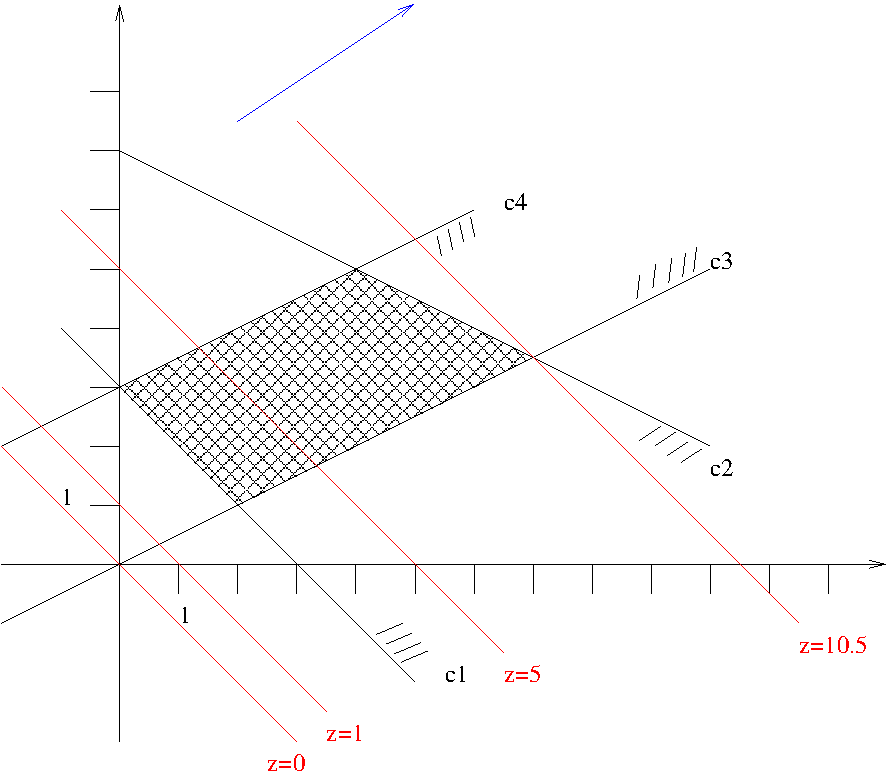
\includegraphics[width=9cm]{Figs/GeomIntuition.pdf}
\end{minipage}
\caption{A simple linear program in two dimensions and its visualization in the
	Euclidean plane.\label{fig:GeomIntuition}}
\end{figure}

Note that it is well possible that the feasible region -- the intersection
of the halfspaces given by the constraints -- is empty. In that case, no solution
exists which satisfies all the constraints, we call the linear program \emph{infeasible}.

\begin{lemma}
If the feasible region is a bounded, non-empty polyhedron, 
the maximum objective function value is 	attained at a corner (also called \emph{vertex})
 of the polyhedron.
\end{lemma}
{\bf Proof:} Follows from the convexity of the polyhedron and the 
linearity of the objective function.

There might be more than one feasible point with maximal objective function value. Think
of respective examples in $2$ and $3$ dimensions.


\subsection{The (Primal) Simplex Algorithm}
Let us now turn to the problem of actually \emph{finding} an optimal vertex of the polyhedron for a given objective function. We will first explain the algorithm in $2$ dimensions and then extend it to higher dimensions.

Without loss of generality let us assume that the objective is to find the \emph{lowest corner} of the feasible region (otherwise rotate the whole problem instance). The high-level strategy of the Simplex algorithm is quite simple:
starting with some corner of the feasible region, jump to a neighboring \emph{lower} corner of the feasible region until all neighboring corners are not below the current corner, see Figure \ref{fig:simplexPrimal}. In two dimensions, there is only one vertex (the highest one) where there is an actual choice which corner to visit next. The other corners -- except the ones with minimum $y$-coordinate -- have exactly one neighboring corner which is lower.

In Figure \ref{fig:simplexPrimal} we also see an example where more than two bounding lines intersect in a vertex (leftmost corner of the feasible region). This is called a \emph{primal degeneracy} and will lead to some complications later on for the Simplex algorithm.


\begin{figure}
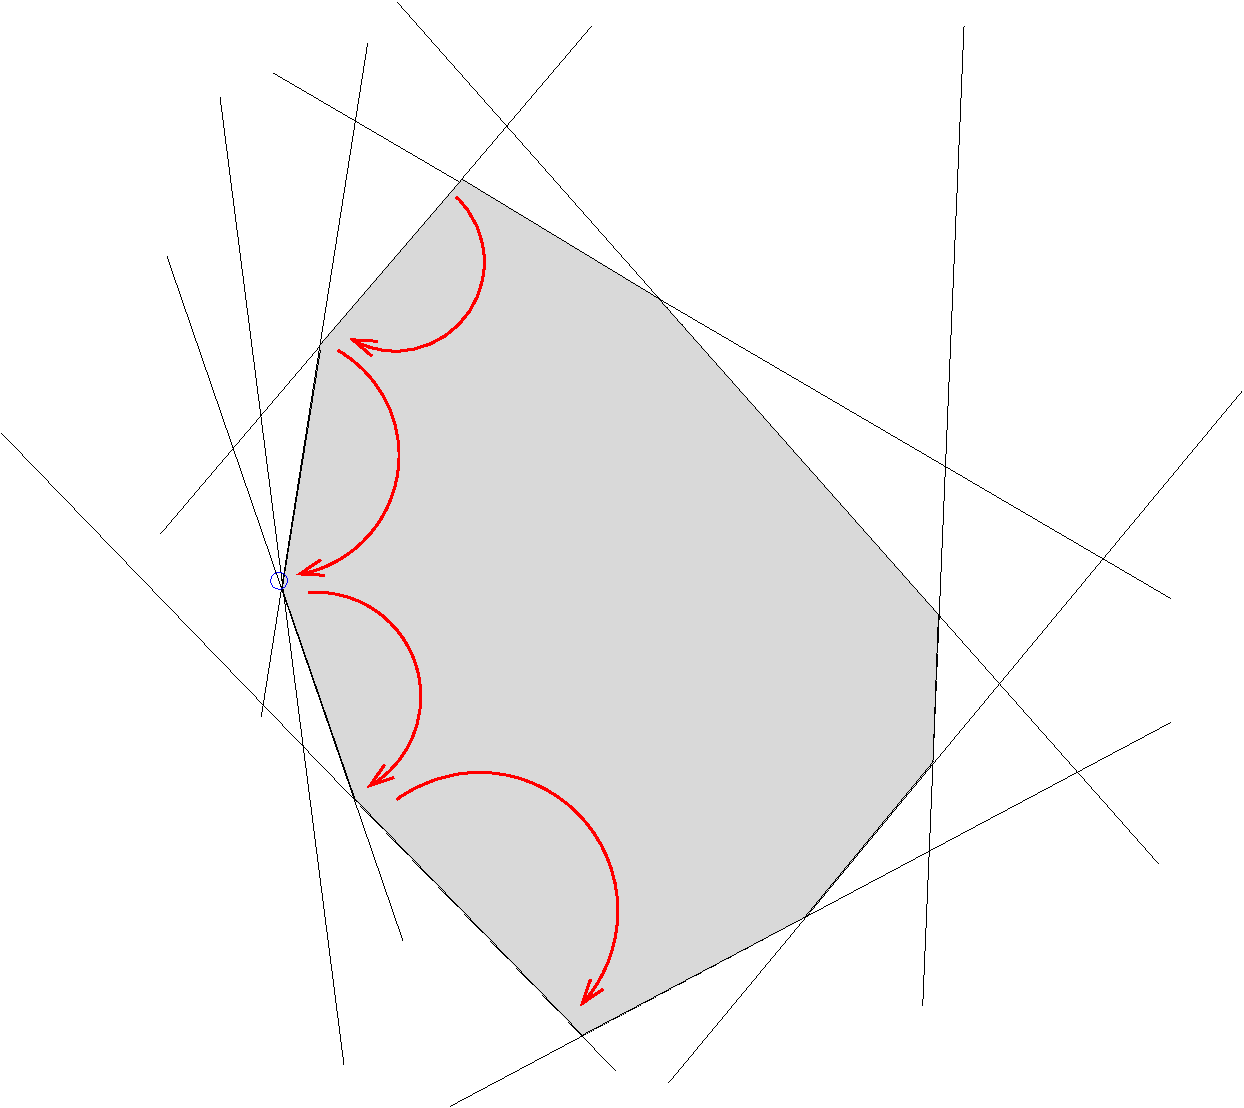
\includegraphics[width=10cm]{Figs/simplexPrimal.pdf}
\caption{Primal Simplex algorithm: jumping from corner to lower corner.}\label{fig:simplexPrimal}
\end{figure}




\subsubsection{Simplex Algorithm in Higher Dimensions}
Translating the basic idea of the Simplex algorithm to higher dimensions is quite straightforward. In $d$ dimensions, a corner of the feasible region is defined by the intersection of $d$ hyperplanes bounding the respective halfspaces corresponding to the constraints (in $\mathbb{R}^3$, three planes in general position intersect in a point). The $d$ hyperplanes defining a vertex/corner are also called a \emph{basis}. The basic strategy remains the same, starting at a corner of the feasible region (defined by $d$ constraints) we keep jumping to adjacent lower corners until there is no neighboring corner below the current curner.

From the description it should be clear that the Simplex algorithm always terminates since for a linear program with $d$ variables and $n$ constraints there can be at most $n\choose d$ corners of the feasible region. As we never visit a corner twice the Simplex algorithm has to terminate after at most $n \choose d$ 'jumps'. Due to convexity of the feasible region, this strategy always leads to the optimal/lowest vertex.

\subsubsection{Making things more concrete}
While the high-level description of the Simplex algorithm seems quite straightforward, there are a few issues which have not been discussed so far:
\begin{itemize}
\item how to compute the corner defined by a basis of $d$ (linearly independent) constraints?
\item how to find an initial \emph{feasible} corner to start the Simplex algorithm from?
\item given a corner, how to find a neighboring \emph{lower} feasible corner if such exists (pivot step)?
\end{itemize}

Consider $d$ constraints $a_i^T x \leq b_i$, $i=1,\dots, d$; the vertex defined by these constraints is the point which satisfies all the constraints with equality, its coordinates can be computed by simply solving the following system of linear equations:
\[
	\mat{a_{11} & \dots & a_{1d} \\ \dots & \dots & \dots \\ a_{d1} & \dots & a_{dd}} x 
		 = \mat{b_1\\ \vdots \\ b_d}
\]

Postponing the problem of finding an initial feasible corner to the exercises, let us now see how we can actually jump from one feasible corner to another, lower feasible corner. This operation is called the \emph{pivot step} and its choice is of great importance for the performance of the Simplex algorithm.

\paragraph*{Pivoting}
Consider a feasible vertex $v'$ defined by $d$ constraints. There are $d$ halflines/rays (each defined by the intersection of $d-1$ constraints) emanating from $v$ on the boundary of the feasible region. We will try to follow one of those rays to get to a lower feasible vertex (which shares $d-1$ constraints with vertex $v$).

Let us first try to figure out which of the $d-1$ halflines to follow to improve our objective function value.
Our current solution is given by $d$ constraints $a_1^Tx\leq b_1 \dots a_d^Tx \leq b_d$. We can write
this system of inequalities as equalities by introducing slack variables $s=(s_1,\dots s_d)\in \setR^d_{\geq0}$:
\[
	\mat{a_{11} & \dots & a_{1d} \\ \dots & \dots & \dots \\ a_{d1} & \dots & a_{dd}} x 
		+ \mat{s_1\\ \vdots \\ s_d} = \mat{b_1\\ \vdots \\ b_d}
\]
We will write this as $A_B x + s = b_B$ in short. The coordinates of the current vertex are determined as 
\[
	x=A_B^{-1}b_B - A_B^{-1}s	
\]
with $s=(0,\dots,0)$, i.e. all $d$ constraints are tight. Moving away from one constraint corresponds to 
increasing its slack variable from zero to some positive value. We want to figure out which slack variable
we can increase to get a higher objective function value. For the objective function we have:
\[
	c^Tx= c^T(A_B^{-1}b_B - A_B^{-1}s)= c^T x' - \alpha_1 s_1 - \dots - \alpha_d s_d
\]
that means expressed in dependence on $s$, the objective function value is a constant (the value at our current
vertex position) and a sum of $s_i$ variables with respective coefficients. If we have for one $i$ 
$\alpha_i<0$, then increasing this slack variable -- i.e. moving away from the corresponding constraint and
sliding along the half-line determined by the remaining constraints -- improves the objective function.
If no such $i$ exists, all neighboring vertices are not below the current vertex.

Now assume we have found a constraint $a_i^T x \leq b_i$
which is going to leave the basis (as we can increase the objective function value thereby). 
It remains to find the constraint which
blocks this movement (if no such constraint exists, the problem is clearly unbounded).

$x'=A_B^{-1}b_B$ is the current vertex, choosing $x''=A_B^{-1}b_B - (A_B^{-1})_{\cdot i}$ (this is a point moved
one unit in the direction we have just determined), we can move 
on the improving ray  ($\lambda\geq 0$)
\[
	\overrightarrow{r}=x' + \lambda \cdot {(x''-x')}
			= x' - \lambda (A_B^{-1})_{\cdot i}
\]
and ask by which other constraint $j$ this movement is blocked first.
We can plug in a point $r(\lambda)$ on the ray in every constraint $l$:
\[
	a_l^{T}(x'-\lambda (A_B^{-1})_{\cdot i})\leq b_l
\]
\[
\Leftrightarrow	a_l^{T}x'-\lambda a_l^{T}(A_B^{-1})_{\cdot i})\leq b_l
\]
If $a_l^{T}(A_B^{-1})_{\cdot i})>=0$ this constraint will never block our movement, otherwise
we obtain the following bound on $\lambda$:
\[
	\lambda \leq \frac{b_l - a_l^{T}x'}{-a_l^{T}(A_B^{-1})_{\cdot i})}
\]
If no constraint gives a bound on our movement, the problem is unconstrained, otherwise the constraint $j$
which determines the smallest upper bound on $\lambda$ is the first constraint hit when moving along
$\overrightarrow{r}$. This constraint enters the basis in exchange for constraint $i$.

\subparagraph*{Pivoting Strategies}
In particular for higher dimensional problems, there are typically \emph{several} constraints for whom moving away from increases the objective function value. There are many strategies to decide which constraint should leave the basis: \emph{the rule of steepest ascent} for example chooses to follow the ray which improves the objective function value at the highest rate; \emph{randomly choosing an improving ray} is another strategy (not as bad as it sounds).

Unfortunately, no strategy is known which guarantees a polynomial number of steps to reach the optimum/lowest vertex. Even worse, for many deterministic pivot rules, there are examples where an exponential number of steps are necessary to reach the optimum (the Klee-Minty cube is a well-known example -- google it!).

\subparagraph*{Basis Cycling and Bland's Rule}

To make things even worse, for many deterministic pivoting strategies there are examples where the Simplex algorithm does \emph{not} terminate at all! This can happen when $d'>d$ constraints intersect in a corner. Here, a naive pivoting strategy might lead to a cycling of the bases never leaving that corner. Bland's rule (google that!) guarantees that after a finite number of steps, the corner is left for a better corner. As applying Bland's rule all the time in practice often leads to worse running times of the Simplex algorithm (more steps), in real-world applicaitons people use rules like the one of steepest ascent and only if cycling is suspected (when the Simplex algorithm stays at the same corner for several steps), Bland's rule is employed until the vertex has been left.

\subsection{Duality}
One very powerful concept in the context of linear programming is \emph{duality}. Let us first look at it in an abstract way and later try to provide some intuition.

Consider a linear program in standard form:

\[
\begin{matrix}
	\max	& c_1 x_1 &+& c_2 x_2 &+& \dots &+& c_n x_n&&\\  
	\mbox{s.t.}	& a_{11} x_1 &+& a_{12} x_2&+& \dots &+&a_{1n} x_n&\leq&b_1\\
			& a_{21} x_1 &+& a_{22} x_2&+& \dots &+&a_{2n} x_n&\leq&b_2\\
			& ..	&&&&&&&&\\
			& a_{m1} x_1 &+& a_{m2} x_2&+& \dots &+&a_{mn} x_n&\leq&b_m\\
\end{matrix}
\]

or more concretely the following linear program (a slight modification of the LP from Figure \ref{fig:GeomIntuition}):
\[
\begin{matrix}
	\max		& x	&+	y	&&\\ 
	\mbox{s.t.}	&-x	&	-y	&\leq&-3\\ 
			&0.5x	&	+y	&\leq&7\\ 
			&0.5x	&	-y	& \leq&0\\
			&-0.5x	&	+y	& \leq&3\\
			&	x	&		& \leq&6\\
\end{matrix}
\]

We could use the Simplex algorithm to solve this LP, but is it possible to give any upper bounds on the objective function value of the optimum solution beforehand?
Consider the two constraints $0.5x+y\leq 7$ and $0.5x-y\leq 0$. We could multiply the first constraint
by $1.5$ and the second constraint by $0.5$ without invalidating them and obtain $0.75x+1.5y\leq 10.5$ and $0.25x-0.5y\leq 0$. Adding these two constraints we get $x+y\leq 10.5$, that is, an upper bound of $10.5$ for the objective function. In this case, this is not the best bound possible, though, since combining
the constraint $0.5x+y\leq 7$ with a multiplier of $1.0$ and the constraint $x\leq 6$ with a multiplier of $0.5$ yields an upper bound of $10$ which happens to be the objective function value of the optimum solution.

A natural strategy to obtain upper bounds on the objective function value is to combine constraints by weighting and adding such that in the sum the coefficients of the variables match the coefficents of the objective function. Note that one better only uses \emph{positive} factors for weighting since multiplication with a negative number turns the $\leq$ into a $\geq$ in the inequality, which renders the obtained 'upper bounds' invalid. More formally we can define the following \emph{dual problem} which formalizes this search for the best upper bound:

\[
\begin{matrix}
	\min& b_1 y_1 &+& b_2 y_2 &+& \dots &+& b_m y_m&&\\  
	\mbox{s.t.}	& a_{11} y_1 &+& a_{21} y_2&+& \dots &+&a_{m1} y_m&=&c_1\\
			& a_{12} y_1 &+& a_{22} y_2&+& \dots &+&a_{m2} y_m&=&c_2\\
			& ..	&&&&&&&&\\
			& a_{1n} y_1 &+& a_{2n} y_2&+& \dots &+&a_{mn} y_m&=&c_n\\
			& y_i\geq 0\\
\end{matrix}
\]
Essentially we have a (positive!) multiplier $y_i$ for each (primal) constraint, $i=1,\dots m$. The multipliers should always be chosen such that the summed coefficients match the coefficients of the objective function; amongst all such multipliers we are looking for the combination which yields the best, that is, the \emph{lowest} upper bound. The discussion so far should has made clear that any feasible solution to this \emph{dual linear program} indeed is an upper bound for the primal linear program. This is also called \emph{weak duality}.

In fact, it turns out that the best upper bound that can be achieved using the dual LP always matches \emph{exactly} the objective function value of the optimum solution in the primal LP. This is called \emph{strong duality}.

\paragraph*{Economic Interpretation of the dual}
Recall our diet-LP from the introduction

\[
\begin{matrix}
	\min	& 7 x_m	&+& 3 x_t&+& 2 x_b&+&4 x_c&&\\  
	\mbox{s.t.}	& 1 x_m &+& 2 x_t&+& 4 x_b&+&1 x_c&\geq&11\\
			& 3 x_m &+& 2 x_t&+& 1 x_b&+&4 x_c&\geq& 7\\
	           	& 5 x_m &+& 0 x_t&+& 0 x_b&+&2 x_c&\geq& 5\\
			& x_i\geq 0\\
\end{matrix}
\]

and let us adopt the perspective of a producer of nutriment pills. He intends to flood the market with carbohydrate, protein and fat fills which are to replace old-fashioned food. The pill producer does know that a typical customer needs to satisfy his need of $11$ units of carbohyrates, $7$ units of proteins, and $5$ units of fat. The pill producer's goal is to set prizes for the pills that maximize his revenue.

There are some constraints, though, which are to be obeyed. For example, if prizes of the pills are so high that buying a one-unit carbohydrate pill, $3$ one-unit protein pills, and $5$ one-unit fat pills is more expensive than $7$ (the cost of one unit of meat), people would rather buy meat instead of these pills.
So let $y_c$ be the price-per-unit that the pill producer wants to charge for the carbohydrate pills, $y_p$, $y_f$ the respective prices for protein and fat pills. The 'meat-constraint' then says that we better have $1 y_c +  3 y_p + 5 y_f \leq 7$ if we don't want people to buy meat instead.
The same holds for true for tofu ($2 y_c + 2 y_p + 0 y_f \leq 3$), bread ($4y_c + 1 y_p +0y_f \leq 2$), and cheese ($1y_c+4y_p+2y_f\leq 4$). The goal is to maximize the revenue for a typical customer who needs $11$ units ob carbohydrates, $7$ units of proteins, and $5$ units of fat, that is, $\max 11y_c + 7y_p +5y_f$. The resulting dual linear program is then:
\[
\begin{matrix}
	\max	& 11 y_c	&+& 7 y_p&+& 5 y_f&&\\  
	\mbox{s.t.}	& 1 y_c &+& 3 y_p&+& 5 y_f&\leq&7\\
			&2 y_c &+& 2 y_p &+& 0 y_f & \leq &3\\
			&4 y_c &+& 1 y_p &+& 0 y_f & \leq &2\\
			&1 y_c &+& 4 y_p &+& 2 y_f & \leq &4\\
			& y_c, y_p, y_f\geq 0\\
\end{matrix}
\]





\end{document}
